\documentclass[uct_visualisation_thesis.tex]{subfiles}

\section{Wprowadzenie}
Algorytm UCT, będący usprawnieniem metody MCTS, jest powszechnie stosowanym algorytmem w sztucznej inteligencji. Analizuje on obiecujące ruchy na podstawie generowanego drzewa równoważącą eksploatację najbardziej korzystnych z eksploracją mniej korzystnych decyzji. Każdemu wierzchołkowi drzewa odpowiada pewien stan rozgrywki, z którego algorytm rozgrywa losowe symulacje, rozszerzając potem drzewo o kolejne możliwe stany. Sposób, w jaki rozrasta się opisywane drzewo, jest kluczowy dla podejmowania przez algorytm obiecujących decyzji.

\section{Cel biznesowy}
Celem projektu jest stworzenie aplikacji pozwalającej na wizualizację drzewa stanów algorytmu UCT. Aplikacja będzie pozwalała na wizualizowanie drzew generowanych podczas rozgrywania dwóch przykładowych gier. Aplikacja powinna pozwalać na wizualizację drzew lub sekwencji drzew. Powinna istnieć możliwość płynnego przybliżania, oddalania i przesuwania drzewa oraz zapisu aktualnego stanu do pliku graficznego. Innymi słowy, wynikiem powinien być produkt, który pozwoliłby zrozumieć klientowi ideę i sposób działania algorytmu UCT.

\section{Założenia projektowe}

\subsection{Założenia funkcjonalne}
Użytkownik korzystający z naszej aplikacji będzie miał do wyboru jedną z dwóch i trzy tryby rozgrywki:
\begin{enumerate}
	\item Gracz versus PC -- użytkownik będzie decydował o swoich posunięciach i zmierzy się on z zaimplementowanym algorytmem,
	\item PC versus PC -- użytkownik będzie świadkiem symulacji algorytmu, który rozgrywa partię z samym sobą,
	\item Gracz versus Gracz -- rozgrywka dwóch graczy, bez wizualizacji.
\end{enumerate}

Zanim jednak przejdzie do rozgrywki, będzie on miał możliwość ustawienia parametrów algorytmu, tj. liczbę iteracji podczas tworzenia drzewa, czy też maksymalny czas na ruch przeciwnika.
Druga opcja, którą będzie dysponować użytkownik, to możliwość wczytania plików reprezentujących drzewa w formacie zarówno binarnym jak i CSV, a następnie możliwość jego dogłębnej analizy. Będzie on mógł wyświetlać informacje na temat wybranego węzła, a także przybliżać i oddalać całą wygenerowaną strukturę. Podczas samej rozgrywki, po wykonanym ruchu przeciwnika gracz będzie mógł analizować drzewo w sposób opisany powyżej, a także wyeksportować je --- będzie miał możliwość zapisania go w formatach wymienionych powyżej, a także w formacie rastrowym. Użytkownik będzie mógł oglądać animację rozrostu drzewa. Powyższe rzeczy dotyczą obu gier w trybach gry z udziałem algorytmu.\\

Aplikacja będzie potrzebować procesora graficznego. Dostęp do sieci nie jest potrzebny dla poprawnego działania aplikacji. \\

Diagram przypadków użycia, który ilustruje przedstawione możliwości, znajduje się na rysunku \ref{rys:usecase}.
\begin{figure}[h!]
	\centering
	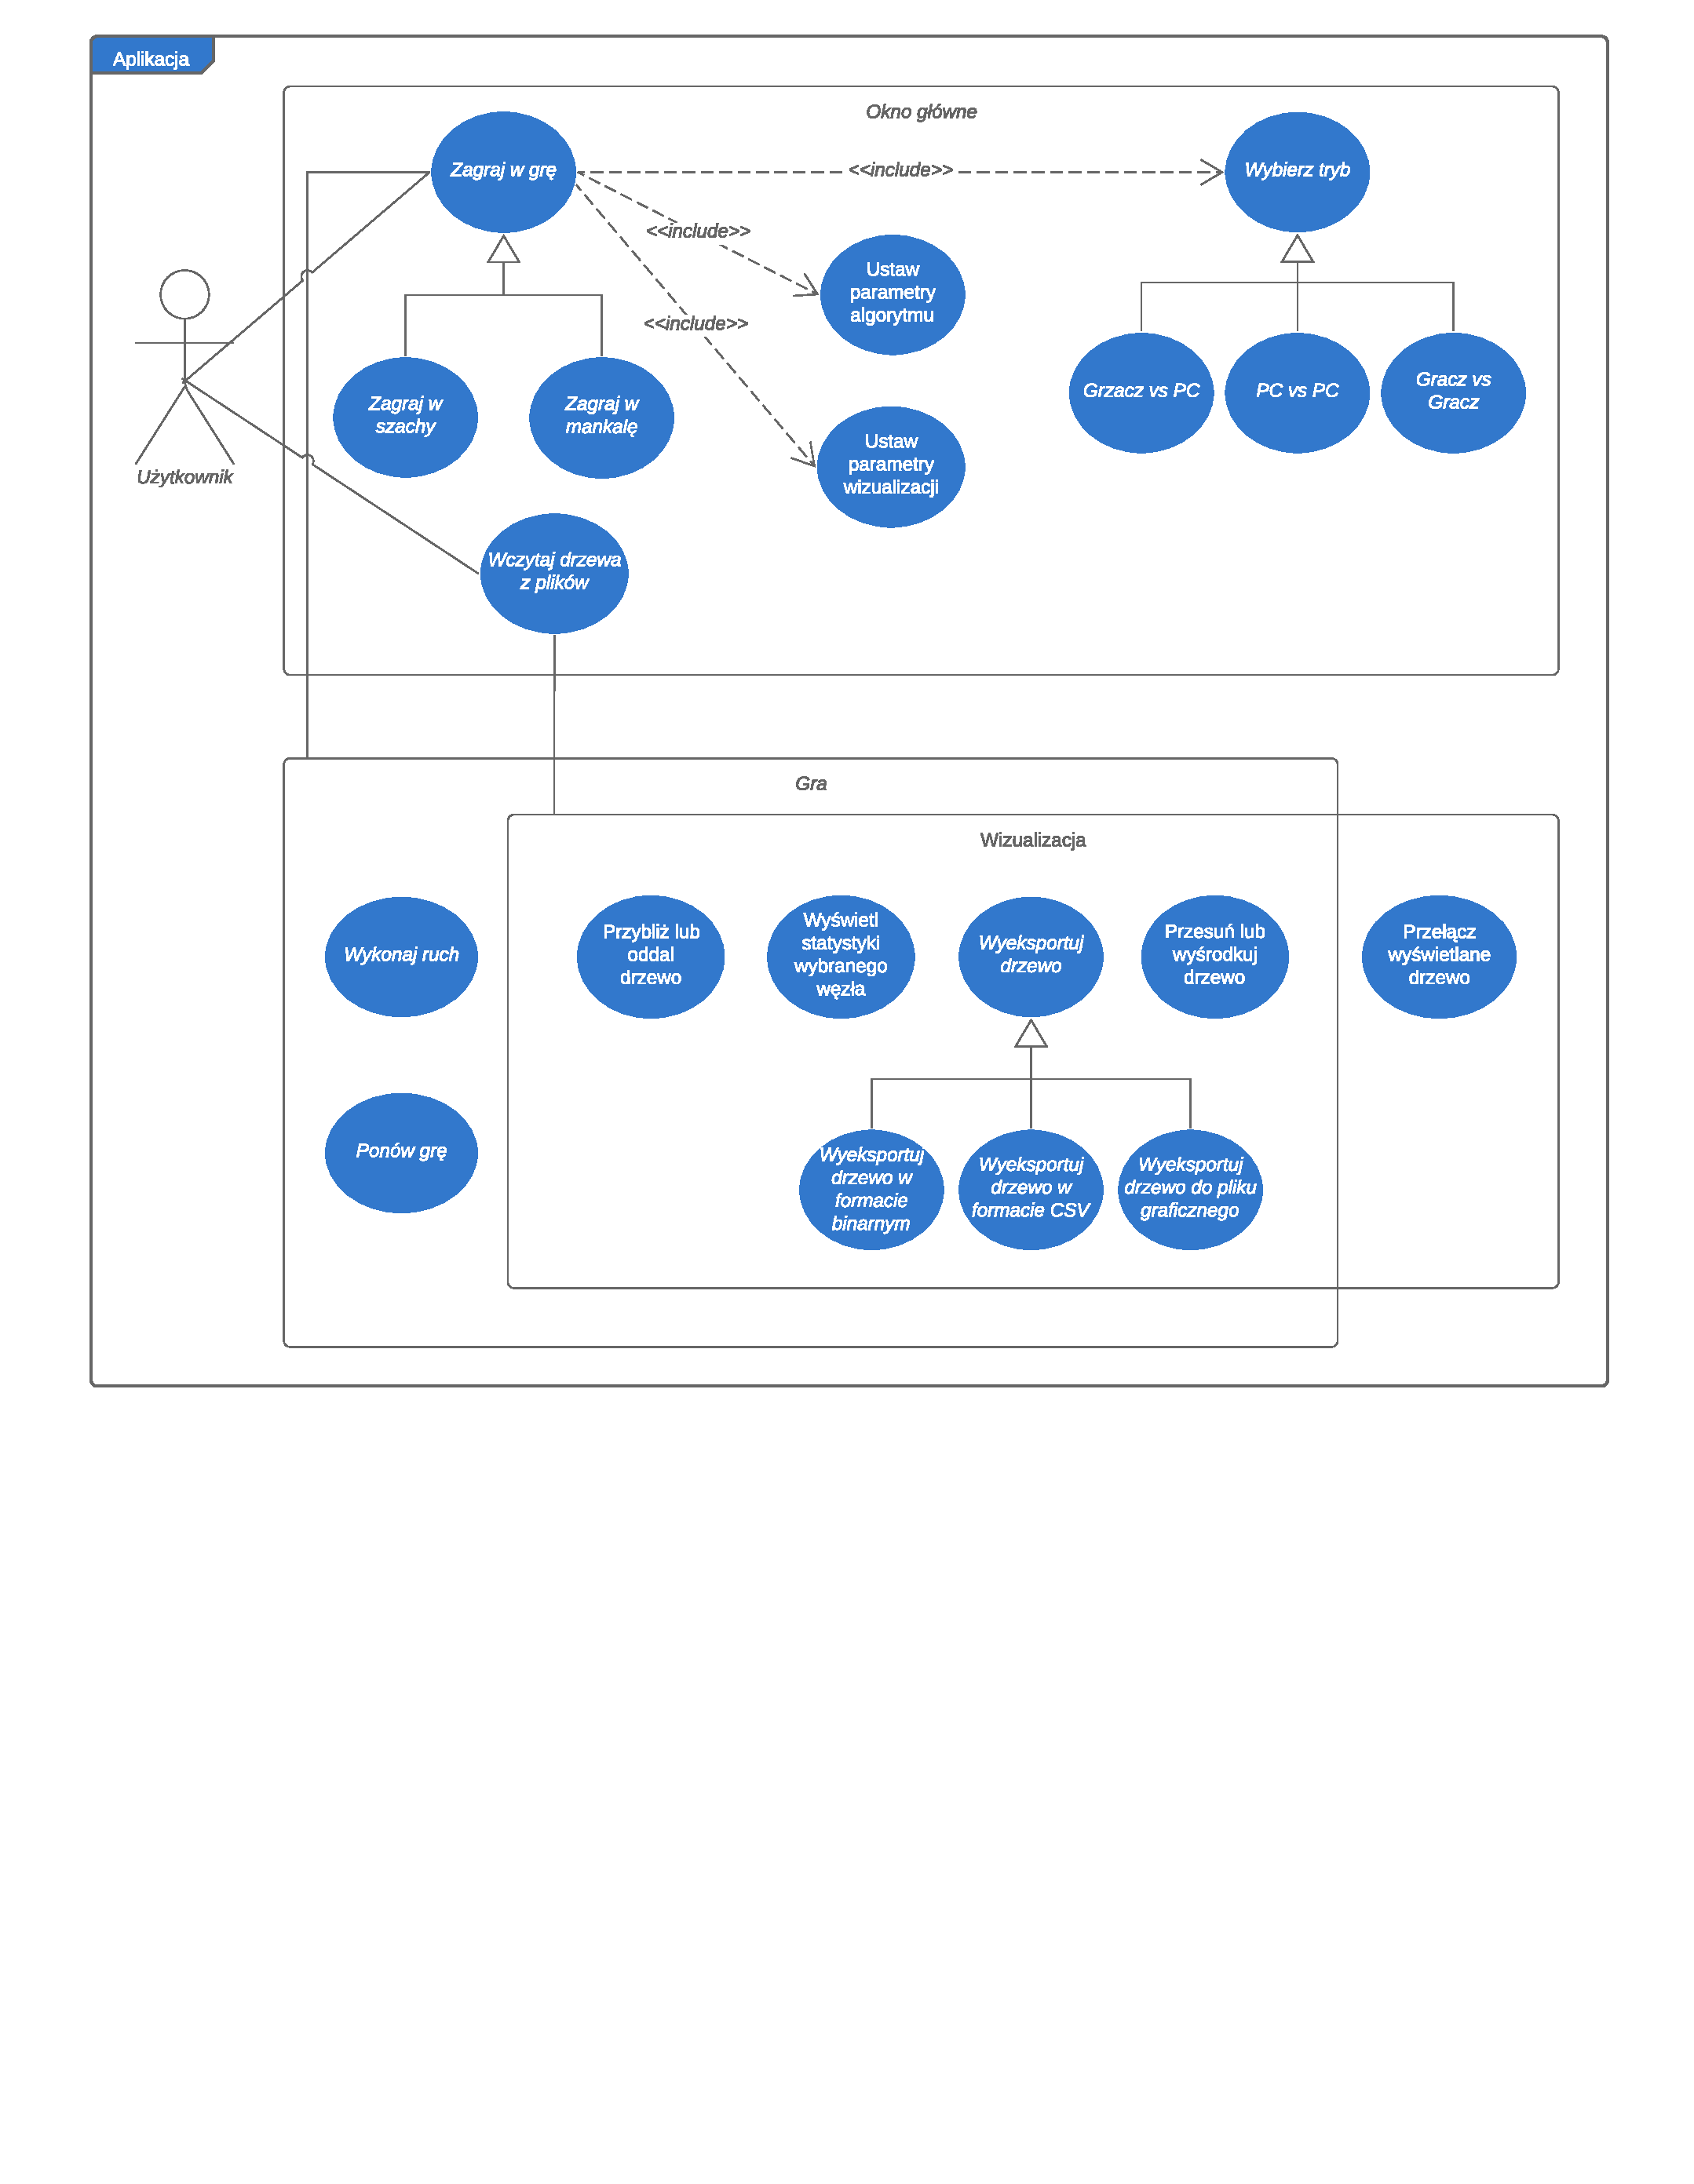
\includegraphics[width=\textwidth, trim={0 6.5cm 0 0},clip]{use-case-simplified-eps}
	\caption{Diagram przypadków użycia}
	\label{rys:usecase}
\end{figure}

\subsection{Założenia niefunkcjonalne}
Wymagania niefunkcjonalne opisane są w tabeli \ref{tab:furps} z użyciem metody FURPS. Zawiera ona opis wymagań sprzętowych aplikacji oraz jej założenia wydajnościowe.

\begin{table}[h!]
	\caption{Analiza FURPS}
	\label{tab:furps}
	\centering
	\begin{tabular}{|l|p{0.7\linewidth}|}
		\hline
		Obszar         & Opis \\ \hline
		Używalność     & Aplikacja działa w jednym oknie wyposażonym w przejrzysty interfejs dla użytkownika. Ponadto, dostarczona jest instrukcja instalacji i obsługi programu.  \\ \hline
		Niezawodność   & Aplikacja działa na komputerze lokalnym i po zainstalowaniu jest dostępna cały czas. Potencjalne błędy nie powinny zamykać aplikacji, a jedynie wyświetlić komunikat dla użytkownika.\\ \hline
		Wydajność      & Aplikacja koryszta głównie z pamięci RAM, procesora i procesora graficznego. Dla drzew do 100 000 wierzchołków wizualizacja nie powinna zajmować więcej niż 3s, a dla 250 000 ---  5s. Wszystkie obliczenia i wizualizacje są przeprowadzane wewnątrz jednej maszyny.\\ \hline
		Wsparcie       & Aplikacja jest przeznaczona dla komputerów z systemami operacyjnymi Windows oraz Linux. \\ \hline
	\end{tabular}
\end{table}